\documentclass{standalone}

\input{tickz_setup.txt}

% Run once then run gnuplot on the .gnuplot generated file to generate a .table aux file that contains the function values 
% Run a second time to generate the plot

\begin{document}
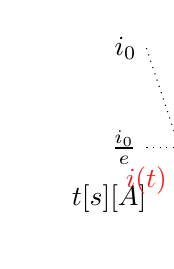
\begin{tikzpicture}[scale=2, samples=100, >=latex]
%%%%%%%%%%%%%%%%%%%%%%%%%%%%%%%%%%%%%%%%%%%%%%%%%%%%%%%%%%
\def\VoltageColor{blue!90!white}
\def\CurrentColor{red!90!white}
\def\PowerColor{green}
%%%%%%%%%%%%%%%%%%%%%%%%%%%%%%%%%%%%%%%%%%%%%%%%%%%%%%%%%%
\PlotAxes{-.2}{2.3}{-.2}{1.5}{$t [s]$}{$[A]$}

\draw (0,1) node[left ]{$i_0$};
%%%%%%%%%%%%%%%%%%%%%%%%%%%%%%%%%%%%%%%%%%%%%%%%%%%%%%%%%%
\draw[color=\CurrentColor, very thick] plot[id=i_chargeVsTime_RC, domain=0:2] function{exp(-3*x)} node[above] {$i(t)$};
\draw[dotted] (0,1) -- (0.3333,0) node[below]{$\tau_s$};
\draw[dotted] (0,0.368) node [left]{$\frac{i_0}{e}$} -- (0.3333,0.368);
\draw[dotted] (0.3333,0.368)  -- (0.3333,0);
\end{tikzpicture}
\end{document}